\section{Building the actual-contract backtester}\label{sec:9}

Historical option quotes, stock prices, rates and dividends come through WRDS. Each source strategy starts with \$10 million. Signal-date contracts trade in the following session if quotes and account checks permit. At full size, put pairs target \$450 vega per IV point on each leg; straddles target \$450 across call and put together. Whole contracts are rounded; put pairs allow an initial vega mismatch of no more than 10\%.


\subsection*{Daily marks, hedges and cash flows}

Options normally remain until expiry. At each close, we mark the existing option and stock positions, record cash flows and then rebalance stock delta. The next day's hedge profit uses the stock held after that rebalance. Final option payoffs and hedge unwinds complete the trade. Trading the same name on later dates is possible subject to existing inventory and risk checks.


Buying hedge stock debits cash; selling it credits cash. The cash balance earns the prior available benchmark rate, with negative cash paying that rate plus one percentage point annually. Short-stock borrow adds 0.30\% annually on short notional. Stock dividends are separate signed cash flows: a long holder receives the dividend and a short holder owes it. The ex-dividend stock-price drop does not replace that cash payment.


Option fills use midpoint plus an adverse charge of 0.10 IV point times traded vega and \$0.03 per contract; stock turnover costs one basis point. Expiry settlement has no option fill charge. Inventory, reserve, stress and quote checks determine admission. A request for less size can pass a pair limit and leave capacity for a later proposal. Appendix~\ref{app:a} defines the checks; they are research assumptions rather than broker margin.


\subsection*{What stays fixed, and what updates?}

\begin{figure}[!htbp]\centering
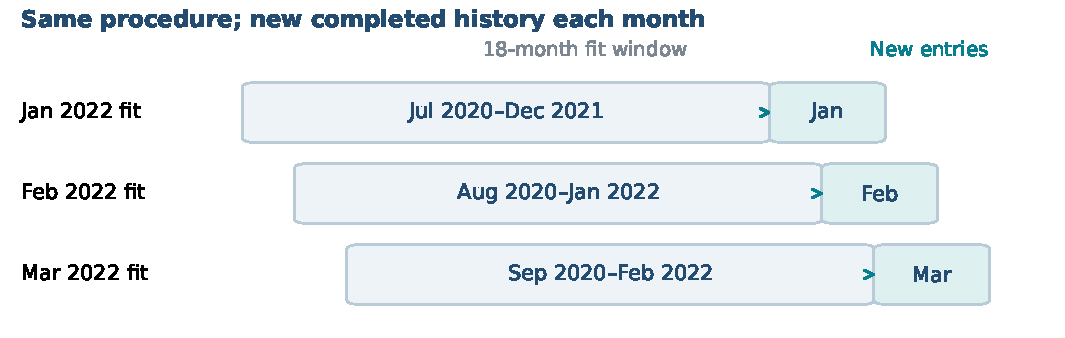
\includegraphics[width=\linewidth]{refit_timeline.pdf}
\caption{Monthly put-policy refitting. Only completed outcomes whose signal dates fall in the displayed 18-month window enter each fit. The selected model settings remain fixed; the tree and size assignments update.}\label{fig:refit-timeline}
\end{figure}

The put inputs, 18-month fitting window, tree settings and 50/75/100\% action menu remain fixed while the tree and size map refit monthly. Only outcomes completed before a fit enter training. A finished March trade can inform an April fit; an unfinished outcome cannot. Straddle and Q fits follow the same timing principle with their own windows. Accounts continue across the 2022 reporting boundary with accumulated cash and positions.


All Sharpe ratios annualize daily returns above cash. Dollar profit subtracts the increase in the continuing cash benchmark; Appendix~\ref{app:e} defines the metrics precisely.


\FloatBarrier
